\documentclass[a4paper]{article}

%% Language and font encodings
\usepackage[english]{babel}
\usepackage[utf8x]{inputenc}
\usepackage[T1]{fontenc}

%% Sets page size and margins
\usepackage[a4paper,top=3cm,bottom=2cm,left=3cm,right=3cm,marginparwidth=1.75cm]{geometry}

%% Useful packages
\usepackage{amsmath}
\usepackage{amssymb}
\usepackage{graphicx}
\usepackage{epstopdf}
\epstopdfsetup{update}

\usepackage[colorinlistoftodos]{todonotes}
\usepackage[colorlinks=true, allcolors=blue]{hyperref}
\usepackage{csquotes}

\title{Reviews and Ratings Verified by Payments on a Blockchain}

\author{
  Chlu
}

\begin{document}
\maketitle

\begin{abstract}

We present a decentralised payments and reputation system that
recognizes vendors for delivering goods and services. Payments made
are accompanied by ratings and reviews and these can be verified by
anyone the vendor grants permission to do so --- in all other cases the
reputation and payments remain private to the vendor. All ratings and
reviews claimed by the vendor can be verified by cross checking data
published on an immutable ledger.

All popular online marketplaces use closed reputation systems, where
users can not take their reputation and sales history to another
marketplace, if they want to. Chlu is an open, decentralised and
freely accessible reputation platform built on top of public
permissionless blockchain. Vendors and customers do not need to put
their trust in any single entity. Anyone can use the Chlu protocols to
make payments, track reputations and verify these reputations once
they have the permission from the vendor to do so.

Chlu provides protocols and open source libraries for marketplaces and
online shops to integrate their payments and reputation systems with
Chlu. The only fees paid are paid to blockchain miners. Vendors on
Chlu own their reputations and use them across any number of
marketplaces, they are not confined to any single marketplace.

\end{abstract}

\section{Introduction}

Marketplaces need reputation to thrive. In real life, and even more so
in online ecosystems the only way for people to do business is to look
at each other's past behaviour and use that as a predictor of their
future behaviour. All popular online marketplaces like eBay, Airbnb,
Amazon marketplace and UpWork include a reputation system that
provides trust in the vendors and in some cases customers
too. However, these marketplaces keep the users' reputations locked to
their platforms, denying users the chance to benefit from reputation
they built. With immutable ledger systems provided by blockchains,
users' reputations can be saved on publicly accessible systems while
being kept private using advanced cryptographic solutions.

It is also important that a vendor's reputation is not publicly
available if a vendor chooses so. Instead, a vendor can choose to
reveal their reputation only to a select customer or on a
marketplace. Vendors can also select marketplaces that can always
display their reputations.

Alongside the reputation system, international payments remain a
challenge. Bank transfers can take weeks and can cost as much as $3\%$
in transaction fees. Blockchains, with their immutable ledgers, have
enabled payment platforms where transfers are near instant with very
low fees. Converting a cryptocurrency to fiat can be as low as $0.26\%$
fee.

Chlu solves the above two problems thanks to blockchains. Using Chlu,
customers can pay vendors within minutes and also record ratings and
reviews associated with the transaction. These ratings, reviews and
payments are saved on the public blockchain. Finally, vendors can keep
their reputations private, such that until they choose to reveal it to
a third party no one can find out a vendor's reputation. This allows
for small vendors to preserve their privacy but reveal it to potential
customers as and when needed.

Chlu provides a trustless and verifiable reputation and payments
system that runs on a public permissionless blockchain. Chlu can be
used by any marketplace to let users build their reputation backed by
payments received, and let the vendors easily use the same reputation
on multiple marketplaces. As vendors receive payments on any of the
marketplaces, the changes to their reputations are visible across all
other marketplaces as well.

Chlu provides a set of protocols that can be implemented by anyone to
enable Chlu into their system. However, we provide reference
implementations for these protocols as vendor and customer wallets as
well as libraries for marketplaces to use on their servers. Our goal
is to drive the growth of an ecosystem around an open, trustless
reputation system.

In the rest of this whitepaper, we demonstrate how important online
reputation is in various industries and elaborate on the problems in
international payments. We then describe how Chlu solves the problem
and how the solution is possible only because of open ledgers provided
by blockchains.

\section{Reputation in Online Marketplaces}

The value of reputation is now a well-established concept when it
comes to eCommerce. The amount of data that we have from companies
like Google, Amazon, eBay and others means that the evidence is
irrefutable. Reviews from our peers are central to how we make
purchasing decisions; this has been clearly established in the
literature\footnote{\url{https://econsultancy.com/blog/9366-ecommerce-consumer-reviews-why-you-need-them-and-how-to-use-them}}.
 
The numbers don't lie when trying to establish the scale of this
opportunity. By 2020, global eCommerce will be a 4 trillion dollar
industry\footnote{\url{https://www.emarketer.com/Article/Worldwide-Retail-Ecommerce-Sales-Will-Reach-1915-Trillion-This-Year/1014369}}. Within
that figure, somewhere around
sixty-one\footnote{\url{https://econsultancy.com/blog/9366-ecommerce-consumer-reviews-why-you-need-them-and-how-to-use-them/}}
percent of consumers read reviews before deciding whether or not to
buy. It could therefore be argued that by the end of the decade, well
over two trillion dollars of eCommerce transactions will be guided by
the current mish-mash of online reviews.
 
Reputation has been at the center of how we make socioeconomic
decisions for millennia. However, we now live in an era where total
strangers who could never attain information about each others'
reputation are nonetheless interacting with each other and engaging in
transactions on a daily basis. This is now commonplace, and yet we
don't really have a good model for establishing the trust needed to
have friction free engagement.
 
Some marketplaces have been very successful at establishing a proxy
for this trust that over time establishes reputation; Amazon, eBay and
others have created somewhat effective walled garden solutions to this
problem with their reviews and ratings systems. We use the term
`walled garden' as the solutions are locked in a closed, managed
ecosystem that is non transferrable externally. In other words, your
reputation on Amazon is useless on eBay. In an ideal world, this would
not be the case.
 
Further distancing the current state of affairs from an ideal model is
the fact that reputation is an umbrella term that doesn't always mean
the same thing from marketplace to marketplace. A given user's
excellent reputation for selling on Amazon may not be a good indicator
of their reputation as an Airbnb user. Even within similar ecosystems,
such as freelancer marketplaces, users can quickly become locked into
a single marketplace due to the sunk cost fallacy. Rachel Botsman
wrote in 2012 for Wired magazine:

\textquote{An aggregated online reputation having a real-world value holds
enormous potential for sectors where trust is fractured: banking;
e-commerce, where value is exponentially increased by knowing who
someone really is; peer-to-peer marketplaces, where a high degree of
trust is required between strangers; and where a traditional approach
based on disjointed information sources is currently inefficient, such
as recruiting}

The need for a universal, open, free-to-use reputation score is
plain. Many businesses have tackled this problem over the last five
years\footnote{\url{http://www.wired.co.uk/article/welcome-to-the-new-reputation-economy}},
and none have truly succeeded. Legit, TrustCloud, Confido, Scaffold,
Reputate are some of the names on corporate headstones in the
reputation economy graveyard.
 
Looking at some of the current players in this space, from established
players like TrustPilot to new entrants like Feefo, and everyone in
between (TrustedShops, Reevoo, and of course even Amazon themselves)
the problem is evident: the current systems are prone to being
gamed. Even a solution like TrustedShops, where `proof of purchase' is
necessary to leave a review, the reality is that ownership of the data
in the purchasing chain is broken several times along the way, and
fake reviews abound. Google uses a long list of independent
vendors\footnote{\url{https://support.google.com/partners/answer/2375474}}
that provide inputs to establish their seller ratings, and still it
appears that approximately
15\footnote{\url{http://www.gartner.com/newsroom/id/2161315}} to
perhaps
35\footnote{\url{https://www.cs.uic.edu/~liub/publications/WWW-2012-group-spam-camera-final.pdf}}
percent of these are still fake. The importance of these ratings
cannot be understated: going from a three-star rating to a five-star
rating gets a business twenty-five percent more clicks from Google
Local
Pack\footnote{\url{https://www.entrepreneur.com/article/295233}}.

Ninety five percent of users doubt the validity of reviews when they
don't see bad scores, and yet Google only shows scores of
three-and-a-half stars or more. Something is broken; customers know
it, and have to resort to personal, highly imperfect hacks to sort the
real review wheat from the fake review chaff.
 
\subsection{So why will Chlu be any different? What has changed?}

The difference today is the emergence of blockchains providing
distributed ledgers, where:

\begin{itemize}
  \item data is stored in a public immutable database; and
  \item payments are publicly visible. 
\end{itemize}

These two key features provide us with tools where trust can be
established in a much more robust manner.

Customers trust other real customers, but existing systems are fraught
with the problem of fake reviews. Using the two essential attributes
of blockchains we can eliminate fake reviews. Customers can only leave
a review and a rating for a vendor if they have made a purchase from
that vendor. Equally importantly, we provide the infrastructure where
payments have to be supported by publicly verifiable requests for
payments from the vendor.

Furthermore, blockchain based payment backed reviews establish a clear
financial inhibitor against fake reviews, and the more the network
grows, the larger this inhibitor becomes.

There can be zero doubt that a truly global, open, free and trustless
reputation system, where you control access to your reputation, in
what context that access is granted, with no third party in the
middle, would revolutionize eCommerce on a global scale. We believe
that the solution that Chlu provides is one of the key components
necessary to take online trade from its current phase into the coming
century where it will inevitably eclipse traditional commerce.

\section{Problems with Online Payments}

In this section we describe the current state of the online payments
market, and why there is a need for a better solution.

\subsection{Current Solutions}

As mentioned above, more and more financial transactions are moving
online with each passing year. E-Commerce in general continues to grow
at double digit rates, and mobile payments are just starting to take
hold in mainstream transactions. You can more than likely pay for your
groceries with your mobile device in your local supermarket today. In
the US, mobile payments rose thirty nine percent in 2016 to reach
\$112bn, according to global firm Forrester Research. The Chinese
market dwarfs these numbers by a factor of almost fifty; third party
mobile payments in China were valued at approximately \$5.5 trillion
last year, which was a turning point for physical retailers accepting
mobile payments in supermarkets, clothing stores and restaurants
leading the way.

Even though there is significant competition in the payments space,
established players, national and international regulators, and other
incumbent factors mean that innovation in payments is uncommon and
generally lags the pace of innovation in technology and the overall
online marketplace. This is especially true for international
payments, where cross border regulation and processes are cumbersome,
costly and ineffective.

Making an international transfer is far from a frictionless
process. The number of steps involved is problematic, often reaching
double digits in both the number of parties involved and the number of
associated fees. This quickly becomes expensive to users of the system
while adding virtually no value other than facilitating the
transaction itself.

\subsection{Fees}

\textquote[Consumers International]{The current industry standard
  allows for opaque pricing, which obscures unfavourable currency
  conversion rates, hides the real cost to the consumer and makes it
  almost impossible for the consumer to `comparison-shop'}

Transaction fees are typically between $2-6\%$ even for intra-bank
transfers, and flat fees are common for international transfers no
matter the transaction size. Typical ranges are between $\$35$ to
$\$65$ per transfer for international outgoing wire transfers
initiated online. Initiating a transfer by other means (e.g.\ over the
phone) will incur further charges on top of this. This pricing may
seem exorbitant, but in reality it is necessary to provide a healthy
profit on top of the long list of fees imposed by the many parties
involved along the way.

The full range of fees that can be applied to standard transactions is
eye-opening: basic transaction fees, chargeback fees, retrieval
request fees, terminal fees, Payment Card Industry fees (of which
there are many), anti-money laundering fees, address verification
service fees, and many, many more. Ultimately, the accumulation of
these hidden fees mean that a given bank may charge anything from four
percent to an incredible fifteen percent for sending money across
international borders.

\subsection{Transaction Times}

Transaction times vary depending again on the type of transfer. For
local transfers, anything from two to five days is typical, and for
international transfers it can take several weeks​ to receive funds at
the destination account. Even for in-country transfers, some eCommerce
payment processors will hold merchants' money for several additional
days due to the greater possibility of chargebacks. This of course
causes real cash flow problems, especially for small businesses.

Of course, there are well known alternatives should speed be of the
essence, but they come at a cost. Users of a service such as Western
Union should expect to pay somewhere between seven to twelve percent
of the total transaction value, making it a very expensive option.

Finally, most current solutions involve trusting a third party to an
extent that adds significant risk to the users of the system. Paypal
is a perfect example of a major payment solution provider that has
repeatedly broken trust with many of its users, locking account access
for seemingly arbitrary reasons, and effectively seizing funds with no
arbitration or review process in place. They have often left
businesses and individuals without access to their funds for six
months or more with zero recourse, and zero oversight. Again, the
current systems are broken, and the world needs a more effective
solution.

\section{Chlu}

In this section we describe the goals of the Chlu protocols and how we
are enabling an ecosystem where anyone can provide a payments and
reputation on their platform. We also explain new ideas about Proof of
Payment (\texttt{PoP}) and Proof of Payment Requested (\texttt{PoPR}).

\subsection{Goals}

Chlu is a decentralised platform for making payments and storing
vendor reputations. Chlu enables vendors to build their reputation on
a decentralised blockchain so they are not confined to a walled garden
of a single marketplace, and customers benefit from a transparent
reputation of vendors backed by payments made for goods and
services. The key goals of a decentralised reputation platform are to
provide:

\begin{description}
\item[Proof of Payment] Customers can leave reviews and ratings only
  if they made a payment to the vendor.  
\item[Proof of Payment Requested] Every payment made can be verified
  to be in response to a payment request by the vendor.
\item[Zero Fees] Chlu does not charge any fees. The only fees in the
  system are those charged by blockchain miners.
\item[Private Feedback] Reviews and ratings are private to the vendor.
\item[All or nothing] Vendors can share their reputation with any
  marketplace, including their own websites.
\item[Multiple Reputation Scores] Vendors cannot hide a review. Once
  they share their reputation with a marketplace their entire history
  is available to the marketplace.
\item[Extensible] Marketplaces are free to compute a reputation score
  for a vendor using the reputation data available.
\item[Open Access] Anyone can use the reputation system as a vendor,
  customer or marketplace.
\end{description}

\subsection{Proof of Payment}

All user feedback for a vendor is tied to payments made by the
customers leaving the rating and review. This is an important aspect
of a trustless decentralised reputation system. \emph{There is no
  third party involved}. Instead of trusting a payment gateway or the
vendors themselves, Chlu ties the rating and review to a payment made
through a trustless payment system.

A customer can leave feedback for a vendor only if there is a
verifiable payment made by the customer to the vendor. Further still,
the customer can leave only one feedback per purchase made. The
customer can update this feedback for upto two months after the purchase.

\subsection{Proof of Payment Requested}

All payments made to a vendor have to be backed by a payment request
signed by the vendor or by the marketplace on behalf of the
vendor. Chlu protocols require that this proof of payment requested or
\texttt{PoPR} is verified before a review is included in the vendor's
reputation.

The requirement of checking for a \texttt{PoPR} avoids an attack by a vendor's
competition to leave negative reviews for the vendor. Even if the
competitor is willing to pay the price of spamming a vendor, the
vendor can put a “flow control” on the reviews received by controlling
the inventory on sale.

\subsection{Zero Fees}

The Chlu protocols are designed so that no third party can directly
profit from facilitating a trustless reputation system. That is, there
are no fees charged for providing the libraries that together make up
Chlu. Even the founders of Chlu can not charge any fees for use of the
system.

The only fee charged is that by miners to save the payment on the
blockchain.

\subsection{Private Feedback}

The reviews and ratings left for a vendor are saved after encrypting
it with the vendor's public key, so that only the vendor can read the
feedback. The vendor can enable sharing of their reviews and ratings
with one or more marketplaces as they see fit.

This requirement is important to avoid marketplaces listing vendors as
members of the marketplace without permission from the vendor as well
as providing privacy to the vendor in case they want to disable any
reviews and ratings for their services.

This feature also allows a vendor to leave a marketplace and thus stop
sharing their reputation with the marketplace, even though the
reputation already shared could have been saved by the marketplace.

\subsection{All or Nothing Reputation}

A vendor can not selectively hide any of the reviews and ratings
received. Once a vendor shares their reputation with a marketplace all
the reviews and ratings are made available to the marketplace. The
marketplace can detect if the vendor is not revealing any of the
reviews and ratings and thus refuse to show the vendor's reputation on
the marketplace, or even further, block the member from the
marketplace outright.

\subsection{Multiple Reputation Scores}

Marketplaces are free to compute vendors' reputation scores based on
their own algorithms. This is important so that marketplaces can
encourage vendor behaviour they choose. For example, some marketplaces
want to track a vendor's average ratings over the lifetime of the
vendor, while others give additional weight to more recent ratings
received.

\subsection{Open Access}

Anyone can join the system as a customer, vendor or a marketplace. No
vetting by third party is required, no minimum balances in a bank
account, or any such old world measures. In this truly open and
decentralised reputation system, there will be no central party that
controls access to the system.

\subsection{Extensible}

Different marketplaces will need to store details of a review as part
of the review created by the customer. For example
Airbnb\footnote{\url{https://www.airbnb.com/help/article/13/how-do-reviews-work}}
and
Homeaway\footnote{\url{https://help.homeaway.com/articles/How-do-I-submit-a-review}},
both property rentals marketplaces, ask their users to review the host
and the property using different criteria. Chlu supports storing any
details a marketplace wants to include in the reviews details by
describing an open reviews structure as part of the Chlu protocols.

\section{Architecture}

\begin{figure}
\centering
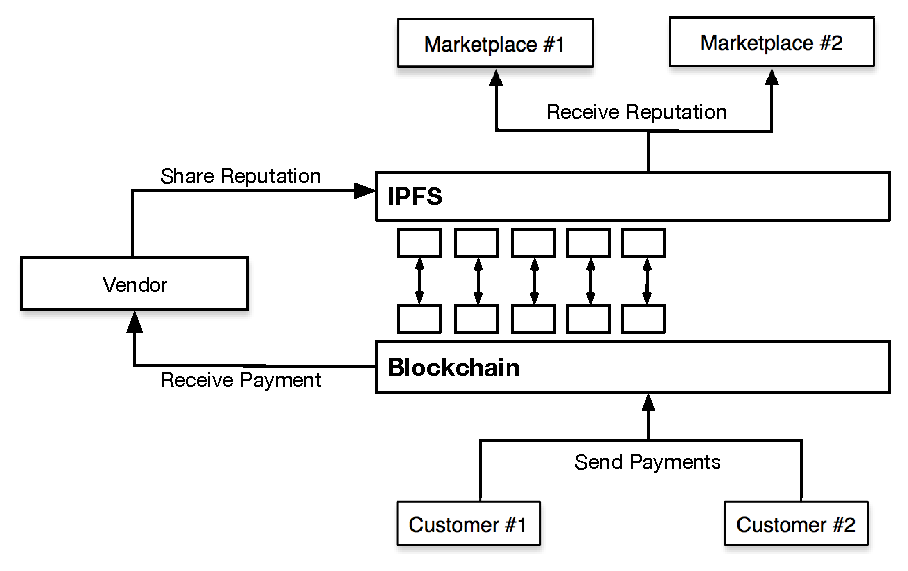
\includegraphics[width=0.5\textwidth]{../reputation.eps}
\caption{\label{fig:reputation}Linking reputation data to payments on blockchain}
\end{figure}


The Chlu platform uses a blockchain to make payments and saves the
\texttt{Proof of Payment} along with a \texttt{Proof of Payment
  Request} in IPFS\cite{ipfs}, a decentralised immutable storage for
objects and files. The key idea behind Chlu is that we can save a
review on IPFS and save the review's IPFS content address in the
blockchain transaction.

Once we have a way to find an immutable review associated with a
payment, we then use cryptography to make sure of the following:

\begin{enumerate}
\item The review is only readable by the vendor
\item The review and the payment associated with it are in response to a payment request created by the vendor or on behalf of the vendor by a marketplace
\item Vendor can't hide any of the reviews they have received
\end{enumerate}

In the following sections we explain in detail how these
characteristics are provided for by the Chlu protocols.  First, we
describe the structure of the payment record first and then describe
the IPFS record structure as well.

\subsection{Proof of Payment Request, \texttt{PoPR}}
The \texttt{Proof of Payment Request} is stored on IPFS and the IPFS
content address for this record is stored inside a payment record.

The record has the following structure:

\begin{description}
\item[$I$, Item ID] A unique ID for the item from the marketplace or the vendor's site
\item[$In$, Invoice ID] The ID of the invoice generated by the marketplace or the vendor's site
\item[$C$, Customer ID] The user ID of the customer on the marketplace if available
\item[$T$, Timestamp] A unix timestamp for when the payment request was generated
\item[$Cr$, Currency] The currency symbol of the blockchain
\item[$A$, Amount] In blockchain currency 
\item[$M$, Marketplace] The domain name of the marketplace
\item[$K$, Key location] The IPFS content address where the public key
  to verify PoPR is published. See section~\ref{sec:key-distribution}
  for details on how vendor gets this key.
\item[$S$, Signature] Signature of all of the above, signed by the
  marketplace's private key for the
  vendor. Section~\ref{sec:key-distribution} describes how this key
  should be generated and stored by the marketplace
\end{description}

$\texttt{Proof of Payment Request}, \texttt{PoPR} = (I, In, C, T, A,
M, Sig(I,In,C, T, A, M))$. The signature is created using $S_v$, the
vendor's signing key the vendor has shared with the marketplace.

\subsection{Payment Record}

The payment record stored on blockchain contains the following
details:

\begin{description}
\item[$V$, Vendor address] The address of the vendor on the blockchain
\item[$A$, Amount paid] In the blockchain currency
\item[$RR$, Review Record] The IPFS content address where the review
  is stored
\end{description}

$\texttt{Payment record}, \texttt{PR} = (V, A, RR)$


\subsection{Review Record stored in IPFS}
  
The reviews stored on IPFS include the following details: 

\begin{description}
\item[$R$, Rating] An integer in the range 1 to 5
\item[$Rv$, Review] A plain text review
\item[$Dr$, Detailed Review] A JSON formatted review; the structure of
  the review is defined by the marketplace
\item[$PoPR$, Proof of Payment Request] This is the request for
  payment signed by the vendors secret key so that it can be verified
  by a vendor public key
\item[$H$, Hash]: The hash of all of the above, $H(R, Rv, Dr, PoPR)$
\end{description}

$\texttt{Review Record}, \texttt{RR} = (PoPR, H, E_v(Pve, (R, Rv, Dr)))$

All the elements of the RR are encrypted using the Vendor's public key,
$P_{ve}$.  The hash along with the encrypted data is stored on IPFS\@. The
content address of the \texttt{Review Record} is stored in the payment
transaction.

\subsection{Key Distribution}\label{sec:key-distribution}

Before we describe the protocols, we describe how keys are distributed
for the signature in the \texttt{Proof of Payment} and the encryption
of the \texttt{Review Record}.

There are a number of systems proposed in literature that describe a
decentralised PKI so that anyone can publish their public keys,
associate the keys with their identity and let them be easily
discoverable. Some excellent proposals that will solve our problem of
key distribution are under
development\cite{blockstack,fromknecht2014decentralized,kulynychdecentralizing,rwot-dpki,IKP,morselli2006keychains},
of these only Blockstack is in production use, however a standalone
API or specifications are not available yet. We will update the Chlu
protocol once a widely adopted decentralised PKI is available. Such a
decentralised PKI will allow third parties to provide an
implementation and does not require Chlu to be developed only for that
one ecosystem.

Until decentralised PKIs are available for production use and can be
easily deployed by marketplaces, Chlu specifies the use of
\texttt{.well-known}\cite{wellknown} location to publish the
marketplace root certification keys. The access to the
\texttt{.well-known} will be made using SSL and therefore our solution
depends on the centralised PKI based on Certification Authorities. We
have chose this approach to provide a pragmatic workable solution that
can be deployed today. However, as we said earlier, once decentralised
PKIs are available in production, Chlu will switch to one with the
easiest adoption curve for marketplaces.


We use IPFS and IPNS to enable key distribution. The key idea is that
marketplaces generate a root key pair and publises is using
DANE. Later, when vendors signup to the marketplace, it generates a
key pair for each vendor, keeps the private key safe, signs the public
key for the vendor and sends it to the vendor. At the moment, the
signature is simple ECDSA and does not include any other meta data. We
describe the details of this scheme in the next section, first need to
defined the key pairs that need to be generated and distributed.

\begin{description}

\item[$S_v$ and $P_v$ is the vendor signing key pair] The marketplace
  generates vendor uses the private key $P_v$ to countersign keys
  generated by the marketplace for signing \texttt{PoPR} on behalf of
  the vendor.
  
\item[$S_{vm}$ and $P_{vm}$ is a signing key pair for vendor $v$ at
  marketplace $m$] When a vendor registers at a marketplace, it
  creates a key pair for the vendor, keeps the secret key, $S_{vm}$,
  safe, signs the public key, $P_{vm}$, using its own root key and
  sends the public key to the vendor. This public key is later used
  validate that the marketplace requested a payment on behalf of the
  vendor.

\end{description}

There is yet another key that is required by the vendor to receive
reviews that are encrypted so that they remain private to the
vendor. The vendor can later decrypt the received reviews and share
them with any marketplace.

\begin{description}
  
\item[$S_{ve}$ and $P_{ve}$ is the vendor's encryption key pair] The
  secret key, $S_{ve}$, is retained by the vendor and the public key,
  $P_{ve}$, is made available over IPNS\cite{ipfs}. This enables the
  vendor to control who can view the review details. To share the
  review details, the vendor can decrypt the reviews and use a
  marketplace API to send them to the marketplace servers.
  
\end{description}


%% Algorithm here
\begin{itemize}
\item Marketplace $\mathbb{M}$ generates a 
\end{itemize}

\subsubsection{Key Revocation}\label{sec:key-revocation}

\subsubsection{Sharing the Vendor Signing Key}

The vendor signing key, $S_v$, is shared with the marketplace by the
Vendor's wallet. The vendor's wallet will create a signing key for
each marketplace where the vendor wants to use Chlu.

Vendor's wallet contains $((M_1, S_{v1}, P_{v1}), (M_2, S_{v2},
P_{v2}), (M_3,S_{v3},P_{v3}), \ldots)$. Where $M_1$, $M_2$, $M_3$ are
names of the various marketplaces the vendor is registered with, and
$S_{vi}$, $P_{vi}$ are the secret and the public keys the vendor has
for the marketplace $M_i$.

The public key, $P_v$ --- required to verify if the signed payment
request is valid --- is saved in a publicly accessible location by the
vendor's wallet. Chlu requires that this key is saved under
\texttt{/ipns/vendorname/chlu/keys/pubver/mi/}. By using IPNS the vendor
can add new keys under the pubver directory and change the IPNS name
to point to the updated Chlu directory under the vendorname IPNS
entry.

Publishing $P_v$ in a well known location helps us provide a useful
property that whoever controls \texttt{/ipns/vendorname/} directory can
publish other keys under that directory and we can be sure all those
keys are owned by the same entity --- in our case the vendor.

\subsubsection{Sharing the Vendor Public Encryption Key}

We now require that vendor's wallet generates an encryption key pair
($S_{ve}$, $P_{ve}$) and publishes the public key Pve under the same
IPNS location as where the signing key was published ---
\texttt{/ipns/vendorname/}.

By requiring that the vendor encryption public key, $P_{ve}$, and the
signature verification key, $P_v$, both be published in the same IPNS
location, we are able to guarantee that the entity who signs the
\texttt{Proof of Payment Request} is the only one that can decrypt the
\texttt{Review Record}.

Once the \texttt{Review Record} is decrypted by vendors, they can then
share the reviews with any marketplaces they want. This guarantees
that the \texttt{Review Record} are private to the vendor until the
moment the vendor decides to share them.

\begin{figure}
\centering
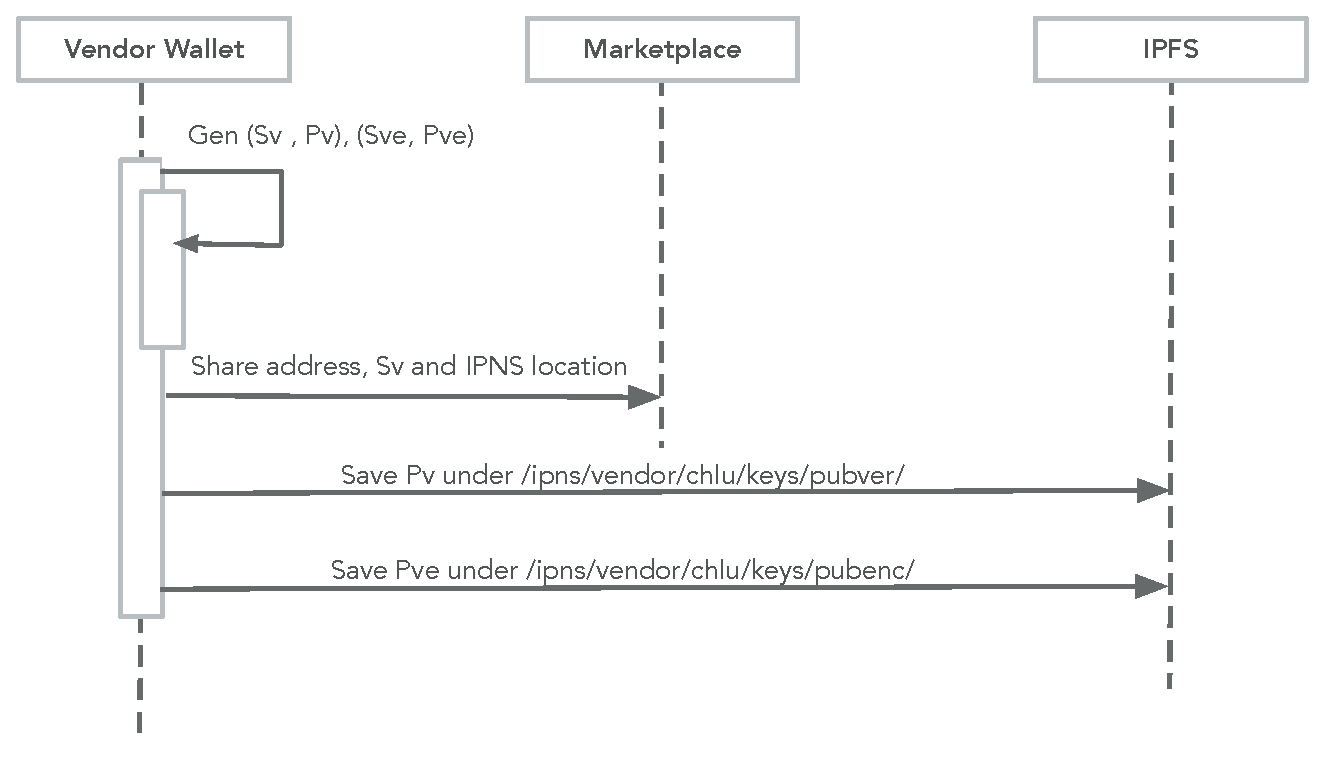
\includegraphics[width=0.6\textwidth]{../vendor-wallet-init.eps}
\caption{\label{fig:vendor-wallet-init}Key distribution: Vendor}
\end{figure}

Figure\ref{fig:vendor-wallet-init} shows the sequence diagram for
generating vendor's signing and encryption keys and publishing them on
IPNS\@.

\subsubsection{Making Payments and Saving Review Records}

We now describe how payment processing works so that the each
published review is supported by a \texttt{Proof of Payment} and each
payment received is in turn supported by a \texttt{Proof of Payment
  Requested}.

When a customer selects an item and wants to make a payment, the
marketplace first generates a \texttt{PoPR} and shares it with the
customer. The customer opens the payment request in a customer wallet
and this payment request includes the \texttt{PoPR}. The customer then
chooses to make the payment, and includes review and a rating as part
of the payment. The customer's wallet makes a blockchain transaction
to make the payment to the vendor and embeds the following two IPFS
content hashes in the payment record.

\begin{description}
\item[PoPR] This is the address of the \texttt{PoPR}, so that anyone who finds
  this transaction on the blockchain can look up the \texttt{PoPR} on
  IPFS and validate it as a payment request made by the vendor.
\item[RR] The \texttt{Review Record} includes the review and rating
  sent by the customer and saved on IPFS. The content address of the
  \texttt{Review Record} is also saved inside the blockchain payment
  record allowing anyone to find the review left for the vendor with
  the payment. The \texttt{RR} also contains a content hash in
  plaintext, and the vendor has to include this hash whenever they
  publish the review to a marketplace. This allows anyone to verify
  that a review is backed by a \texttt{Proof of Payment}, which in
  turn is backed by \texttt{Proof of Payment Requested} as shown
  earlier, and the review has not been tampered with.
\end{description}

\begin{figure}
\centering
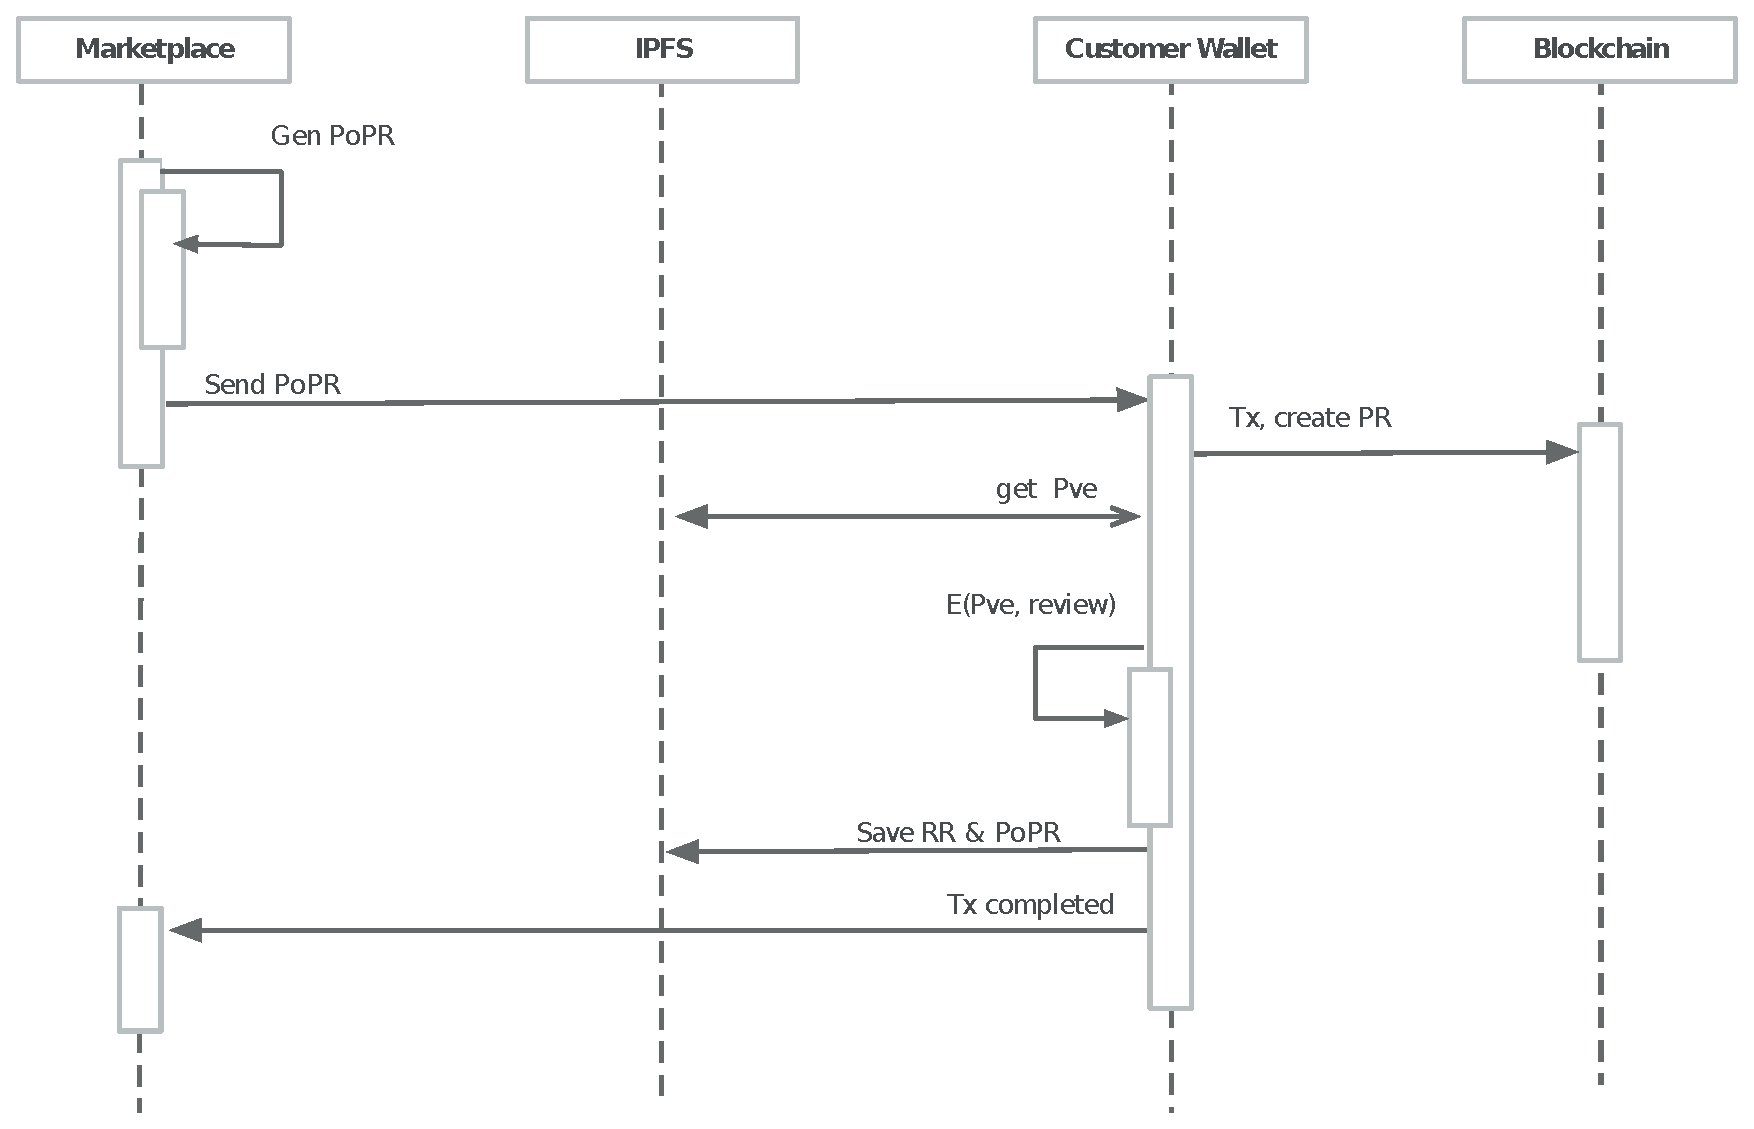
\includegraphics[width=0.6\textwidth]{../payment-processing.eps}
\caption{\label{fig:payment-processing}{Payment Processing}}
\end{figure}

Figure\ref{fig:payment-processing} shows how marketplace and the
customer wallet interact to save the \texttt{PoPR}, \texttt{PR} and
\texttt{RR} when a payment is made to a vendor selling products or
services on the marketplace.


\subsubsection{Verifying Reviews}

Vendors are free to share their review history with marketplaces and
send an update to the marketplace when a review is available. We show
how a marketplace can verify that the \texttt{Review Record} submitted
by a vendor has not been modified by the vendor since it was
published.

There are a few important elements of \texttt{Payment Record} and
\texttt{Review Record}:

\begin{enumerate}
\item \texttt{Payment Record} contains the IPFS content address of a
  \texttt{Review Record}.
  
\item Each \texttt{Review Record} is encrypted using $P_{ve}$, the
  public encryption key of the vendor. This key is owned by the owner
  of $P_v$ whose corresponding $S_v$ signed the \texttt{PoPR}.

\item Each \texttt{Review Record} has two parts to it, the hash of the
  plaintext and the encrypted review.
\end{enumerate}

Once a marketplace has the above information, it can take a hash of
the plaintext review submitted by the vendor and compare it to the
hash included in the \texttt{Review Record}.

This is, however, not enough to make sure the review is valid. We need
to further verify that the \texttt{Proof of Payment Request} is also
signed by the vendor who controls the same location where the public
key $P_v$ was stored to encrypt the \texttt{Review Record}. The
following sequence of steps help marketplaces verify the review has
not been changed by the vendor and is a valid review for the vendor.

\begin{enumerate}
\item Marketplace fetches the \texttt{PoPR} and $P_v$ for the vendor
\item Marketplace validates that the signature for \texttt{PoPR} can be
  verified using $P_v$
\item Marketplace then fetches the \texttt{Review Record}, \texttt{RR}
  that it wants to verify
\item Marketplace finds the plaintext \texttt{RRv} with the same hash that
  vendor has submitted
\item Marketplace takes a hash of the plaintext part of \texttt{RRv}
  and compares it to the hash in the \texttt{RR}
\item If the above two hashes are the same, the marketplace is sure
  that vendor is in control of the private key whose public key is
  saved in the same IPNS directory where the $Pv$ is stored
\end{enumerate}

\begin{figure}
\centering
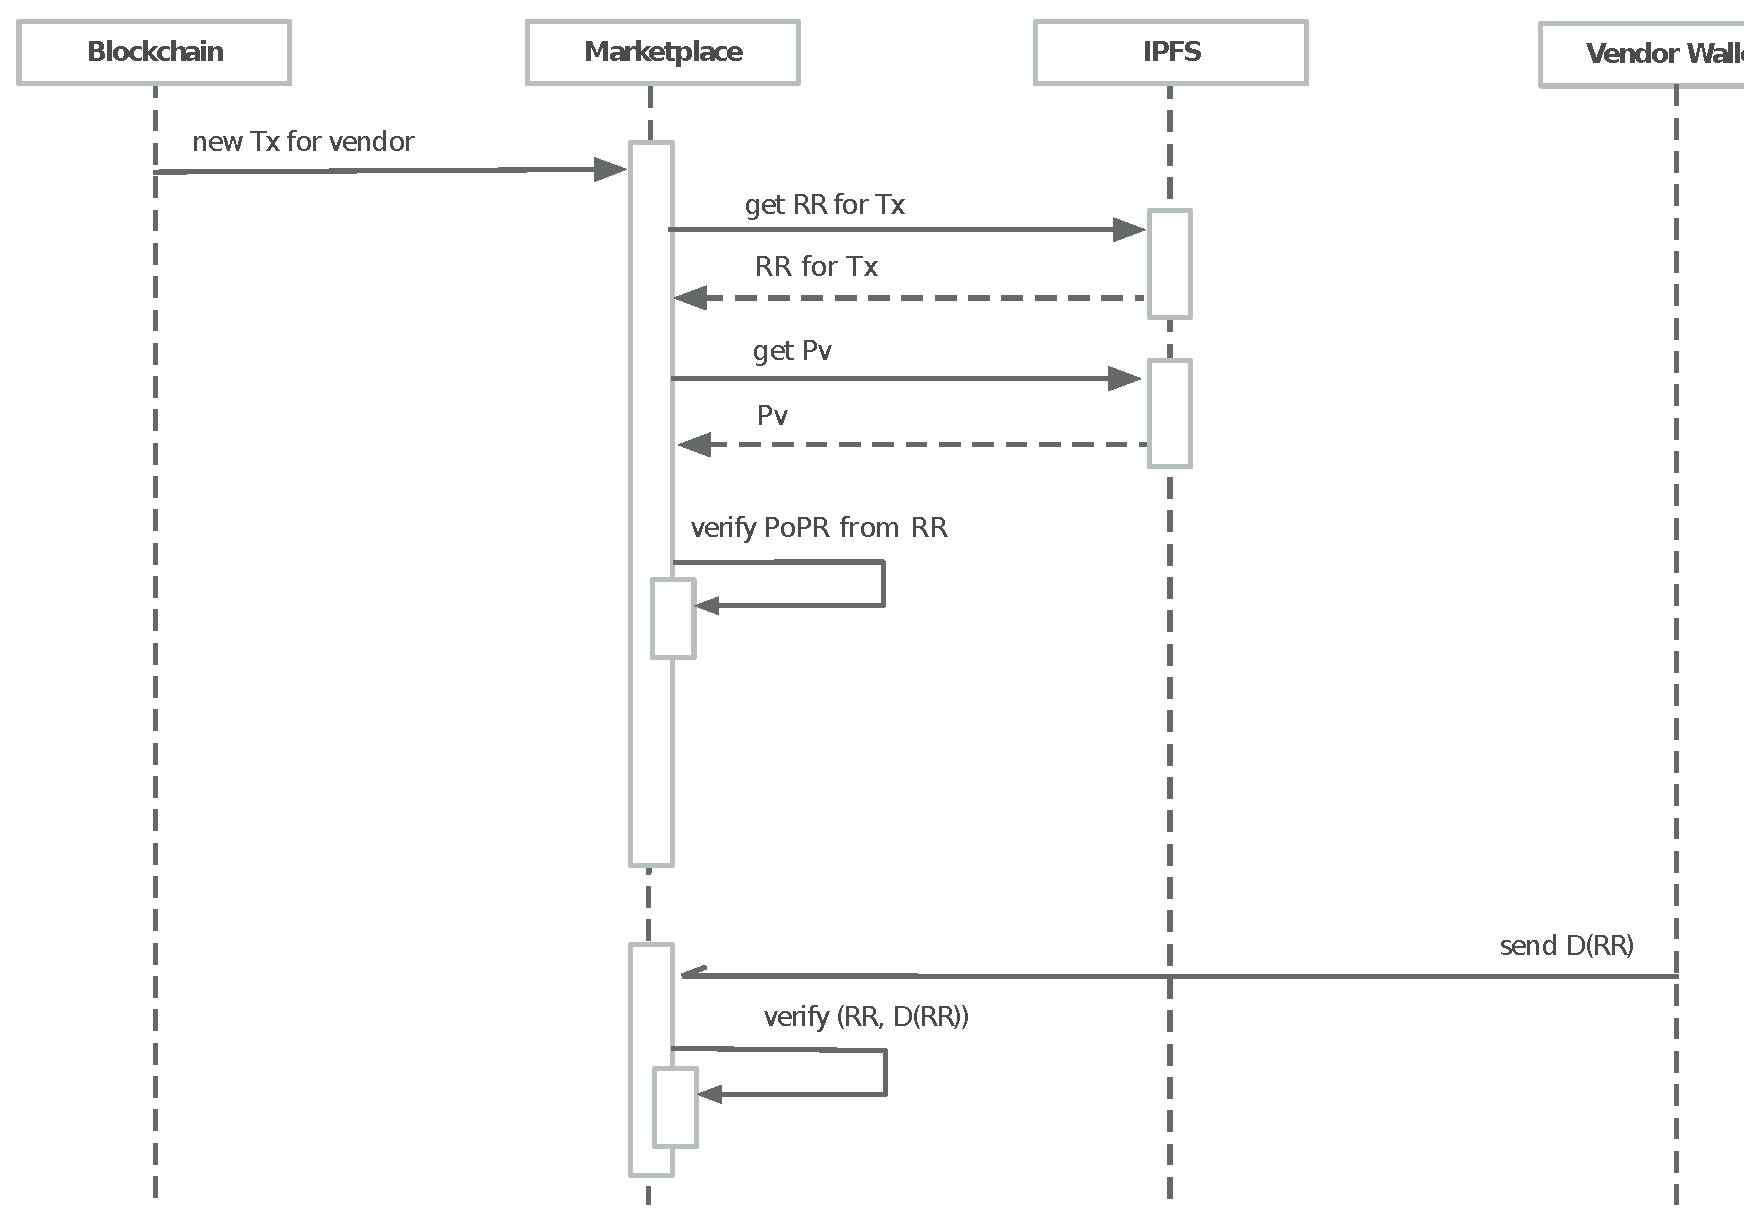
\includegraphics[width=0.6\textwidth]{../validating-new-tx.eps}
\caption{\label{fig:validating-new-tx}Validating reviews found from blockchain transactions}
\end{figure}

Figure\ref{fig:validating-new-tx} above shows the sequence of actions
for review verification.

The above process assures the marketplace that the same vendor is in
control of $S_v$ and $S_{ve}$ and that the vendor has not altered the review
since it was encrypted by the customer wallet using $P_{ve}$.

This section described how vendors can share their reviews with
marketplaces directly using their wallet. It should be noted, however,
that this functionality can be provided by any service that watches
the blockchain for transactions going to the vendor address and shares
the reviews as they come in.

\subsubsection{Review Completeness}

A vendor receieves payment to an address they submit to a marketplace.
Once we show that review completelness property is provided for a
single vendor address it is easy to see how the protocol can be
extended to support multiple vendor addresses. Multiple addresses and
review completeness is easily provided for once we add a requirement
on the marketplaces that they publish all the vendor addresses that
vendors provide them for receiving payments.

To see how review completeness is provided for a single vendor
address. We note that marketplaces can monitor the block chain for any
payments to that address and can find all the \texttt{Review Record}s
for all of those payments.

\subsubsection{Reviews After Product Delivery}

The above solution shows how a review that is created when a customer
makes a payment is shared with marketplaces in a secure way. However,
we still need to allow customers to pay for a product and create a
review after the product has been received, which means separating the
events of payment and writing a review. While trying to address this
separation we can also provide support for customers updating reviews
that they have already created for a given purchase.

As described uptill now, the \texttt{Payment Record} stored on the
blockchain stores a reference to the IPFS content address of the
\texttt{Review Record} authored by the customer. To support the
separation of payments and reviews, and to allow customers to update a
review, we change the requirement of the IPFS content address to
instead be an IPNS name of a directory.

Once the marketplace has access to an IPNS name of a directory from a
\texttt{Payment Record}, it can poll the directory to check if there
is any new data. If new data is available under the directory, IPNS
guarantees that it has been created by the customer who left the first
review. This is achieved by the IPNS requirement that only the holder
of the private key that created the IPNS name can add content to the
location pointed to by the IPNS name.

The above requires a customer wallet initialization similar to the
vendor wallet initialization so that the customer wallet creates a key
pair to be used for saving reviews and publishing an IPNS name.

In future, the requirement from the marketplace to poll an IPNS
directory can be replaced by IPFS pubsub once it is ready for
production release and, more importantly, supports authentication of
pubsub events\footnote{\url{https://ipfs.io/blog/25-pubsub}}.

\subsection{Sybil Attacks}

Any reputation system needs to be resistant to Sybil attacks, so that
no vendors can create multiple customer accounts and give themselves
high ratings through these sockpuppet accounts. A reputation system
can be made resistant to Sybil attacks by requiring high costs for for
using the system or requiring a network of identities within the
system. Since Chlu is free to use it would first appear that it would
be highly vulnerable to Sybil attacks. But there are two important
features that make Chlu resistant to Sybil attacks:

\begin{enumerate}
\item Marketplaces are free to choose how they use a vendor's reputation
  history
\item Marketplaces charge vendor a commission to sell items through
  their service
\end{enumerate}

Keeping the above two points in mind, let us see how a vendor can
conduct a Sybil attack and how Chlu remains resistant to the attacks
thanks to well behaving marketplaces.

Say a vendor launches a Sybil attack by creating numerous fake
customer accounts and tries to gain a positive reputation history. In
this case, the vendor creates a dummy marketplace, that charges no
commissions, generates \texttt{PoPR} for the sockpuppet customers and
makes payments to the vendor's account backed by these \texttt{PoPR},
attaching the best ratings to each payment.

The vendor will succeed in creating a reputation history where each
\texttt{PoPR} is signed by the dummy marketplace, and the vendor could
use this history to show top ratings on their own website. However, any
other marketplace will chose to leave out ratings from this dummy
marketplace. The vendor's ratings on other marketplaces will only show
ratings received on other marketplaces that they accept ratings from.

If vendors try to create sockpuppet accounts on a legitimate
marketplace, they will have to pay commissions of up to 15\% charged
by these marketplaces, the vendor will not be able to leave too many
positive reviews without burning a lot of money.

\section{Which Blockchain}

The system described above can work on Bitcoin and all the blockchains
derived from bitcoin that support the \texttt{OP\_RETURN}
operator. The content addresses for \texttt{Review Record} and
\texttt{Proof of Payment Request} can be saved in the
\texttt{OP\_RETURN} field, as they will together fit into the 80 bytes
limit for \texttt{OP\_RETURN}.

We provide reference implementations for Bitcoin, Litecoin and ZCash,
all of which support \texttt{OP\_RETURN}. As well as on
Ethereum\footnote{\url{https://www.ethereum.org/}} where we store IPFS
content addresses on the blockchain using a thin smart contract.

\section{Comparison}

Chlu is not a marketplace. This immediately differentiates it from all
other efforts to provide decentralised marketplaces. Instead, Chlu is
a service that can be used by any marketplace, decentralised or not.

Chlu is an openly accessible and decentralised service for making
payments and building online reputation as a vendor. We contrast Chlu
with the other decentralised marketplaces to make it clear where Chlu
stands in comparison. In the case where the marketplace does not yet
exist, but is only described on a website, we compare Chlu with the
planned features offered by the marketplace.

The most important features we compare are whether the review and
ratings systems are walled gardens or not, and whether they require
proof of payment for reviews. We also include extensibility as a
property because without it, the reputation system can not be used by
marketplaces that encourage different user behaviours.

If the specifications of the various systems don't provide a clear
answer for these properties, we leave it as unknown.

\begin{center}
\begin{tabular}{ | r | c | c | c | }
  \hline
  System & Walled Garden & Proof of Payment & Extensible \\
  \hline

  Chlu & No & Yes & Yes \\

  \hline

  OpenBazaar\cite{openbazaar} & Yes & Yes & No \\

  \hline

  Ethlance\cite{ethlance} & Yes & Yes & No \\

  \hline

  District0x\cite{district0x} & Yes & Unknown & No \\

  \hline

  Colony\cite{colony} & Yes & Unknown & Unknown \\

  \hline

  Monetha\cite{monetha} & Yes & Yes & No \\

  \hline
\end{tabular}
\end{center}

The above table shows how Chlu's goal of decentralised reputation is
not being provided by any other system.

\section{Conclusion}

We describe Chlu, a decentralised reputation system where the vendors
are in control of the reputation they have earned by selling products
and services on various marketplaces across the internet. Chlu defines
protocols that do not require any trusted third party to run services
or authorise any transactions. Chlu protocols use a blockchain for
making payments, save reviews and ratings on IPFS/IPNS, and use
cryptography to provide a secure system of verifying claims made by
vendors.

In a global economy with products and services bought and sold between
strangers, reputation systems are instrumental in driving
business. However, until now, reputation systems have been enclosed in
walled gardens. Even if vendors have excellent reputations in one
marketplace they are unable to successfully sell products and services
on another marketplace.

Marketplaces also have to constantly fight vendors trying to game
their reputation systems, with Chlu's reputation history backed by a
proof of payment, and no need for a trusted third party required to
verify transactions, all marketplaces will benefit tremendously from
adopting Chlu.

\bibliography{position-paper}{}
\bibliographystyle{plain}

\end{document}
